% !TEX TS-program = pdflatex TEX encoding = UTF-8 Unicode

% This is a simple template for a LaTeX document using the "article"
% class.  See "book", "report", "letter" for other types of document.

\documentclass[11pt]{article} % use larger type; default would be 10pt

%\usepackage[utf8]{inputenc} % set input encoding (not needed with
%XeLaTeX)


%%% Examples of Article customizations
% These packages are optional, depending whether you want the features
% they provide.  See the LaTeX Companion or other references for full
% information.

%%% PAGE DIMENSIONS
\usepackage{geometry} % to change the page dimensions
\geometry{a4paper} % or letterpaper (US) ocher a5paper or....
\geometry{margin=1in} % for example, change the margins to 2 inches
%   all round \geometry{landscape} % set up the page for landscape
%   read geometry.pdf for detailed page layout information
\usepackage{graphicx} 
% \usepackage[parfill]{parskip} % Activate to begin paragraphs with an
% empty line rather than an indent

%%% PACKAGES
%\usepackage{booktabs} % for much better looking tables
\usepackage{array} % for better arrays (eg matrices) in maths
%\usepackage{paralist} % very flexible & customisable lists
%(eg. enumerate/itemize, etc.)
\usepackage{verbatim} % adds environment for commenting out blocks of
%text & for better verbatim \usepackage{subfig} % make it possible to
%include more than one captioned figure/table in a single float These
%packages are all incorporated in the memoir class to one degree or
%another...

%%% HEADERS & FOOTERS
\usepackage{fancyhdr} % This should be set AFTER setting up the page
                      % geometry
\pagestyle{fancy} % options: empty , plain , fancy
\renewcommand{\headrulewidth}{0pt} % customise the layout...
\lhead{}\chead{}\rhead{}
\lfoot{}\cfoot{\thepage}\rfoot{}

%Acknowledgements:  
%We acknowledge the support of Krystle Chavarria and 
%Regina Lamendella for extraction of DNA from Great Prairie soil samples
%and the technical support of Stephanie Malfatti and Tijana Glavina del Rio 
%at the DOE JGI.  Add Eddy.  I'm not sure in what capacity.
%Add GLBRC and NSF $ for Adina
%Add John Johnson & Eric and HPC
%Add any grants for Titus including Amazon

%%% SECTION TITLE APPEARANCE
%\usepackage{sectsty} \allsectionsfont{\sffamily\mdseries\upshape} %
%(See the fntguide.pdf for font help) (This matches ConTeXt defaults)

%%% ToC (table of contents) APPEARANCE
%\usepackage[nottoc,notlof,notlot]{tocbibind} % Put the bibliography
%in the ToC \usepackage[titles,subfigure]{tocloft} % Alter the style
%of the Table of Contents
%\renewcommand{\cftsecfont}{\rmfamily\mdseries\upshape}
%\renewcommand{\cftsecpagefont}{\rmfamily\mdseries\upshape} % No bold!

%\usepackage[T1]{fontenc}
                    \usepackage[latin9]{inputenc}
%\usepackage[active]{srcltx}
\usepackage{setspace}
\usepackage{lscape}
\doublespacing
\usepackage[english]{babel}
\bibliographystyle{naturemag}
 \usepackage{url}



\begin{document}

\title{Assembling large, complex environmental metagenomes}
\author{ACH, JJ, ST, JMT, CTB} 
\maketitle

\section{Introduction}  
Complex microbial communities operate at the heart of many crucial
terrestrial, aquatic, and host-associated processes, providing
critical ecosystem functionality that underpins much of biology
(\cite{Arumugam:2011p735,Hess:2011p686,Iverson:2012p1281,
  Mackelprang:2011p1087,Qin:2010p189,Tringe:2005p174,Venter:2004p170}).
These systems are difficult to study {\em in situ}, and we are only
beginning to understand their diversity and functional potential.
Advances in DNA sequencing technologies now provide unprecedented
access to the genomic content of these communities via shotgun
sequencing, which produces millions to billions of short-read
sequences \cite{Hess:2011p686,Mackelprang:2011p1087,Qin:2010p189}.
Because shotgun sequencing samples communities randomly, ultradeep
sequencing is needed to detect rare species in environmental samples,
with an estimated 50 Tbp needed for an individual gram of soil
\cite{Gans:2005p1365}.  Both the short read lengths and large volume
of sequencing data pose new challenges to sequence analysis
approaches.  A single metagenomic project can readily generate as much
or more data is in global reference databases; for example, a
human-gut metagenome sample containing 578 Gbp \cite{Qin:2010p189}
produced more than double the total content of the 202 Gbp NCBI RefSeq
database (Release 56).  Moreover, short reads contain only minimal
signal for homology searches and are error-prone, limiting direct
annotation approaches against reference genomes.  And finally, the
majority of genes sequenced from genomes contain little or no
similarity to experimentally studied genes, further complicating
homology analysis \cite{Arumugam:2011p735,Qin:2010p189}.

\emph{De novo} assembly of raw sequence data offers several advantages
over analyzing the sequences directly.  Assembly removes most random
sequencing errors and decreases the total amount of data to be
analyzed.  These resulting assembled contigs are longer than
sequencing reads and provide gene order.  Importantly, \emph{de novo}
assembly does not rely on the existence of reference genomes, thus
allowing for the discovery of novel elements.  The main challenge for
metagenomic applications of \emph{de novo} assembly is that current
assembly tools do not scale to the volumes of metagenomic datasets
being generated: metagenomes from rumen, human gut, and permafrost
soil sequencing could only be assembled after sample preprocessing to
discard low abundance sequences
\cite{Hess:2011p686,Mackelprang:2011p1087,Qin:2010p189}.  Traditional
assemblers are designed for single genomes whose abundance
distribution and diversity content are typically simpler than
community metagenomes.  Although many metagenome-specific assemblers
have recently been developed for community asssembly, these assemblers
are limited in terms of the sample sizes they can assemble.
% @CTB cite?

Here, we combine two approaches, digital normalization and
partitioning, to enable large-scale metagenomic {\em de novo}
assembly.  Digital normalization reduces the dataset size by
discarding reads from high-coverage regions \cite{XXX}.  Subsequently,
partitioning separates reads based on transitive connectivity,
resulting in easily assembled subsets of reads \cite{XXX}.  We
evaluate these approaches by comparing unfiltered and filtered
assemblies of a human gut mock community dataset, and find that these
filtering methods result in assemblies nearly identical to assemblies
from the unprocessed dataset.  Next, we apply these approaches to the
assembly of two previously intractable soil metagenomes, one from Iowa
agricultural soil under continuous cultivation, and one from native
Iowa prairie.  We compare the predicted functional capacities and
phylogenetic content of the assembled contigs and conclude that despite
significant phylogenetic differences, the functions encoded in both
soil data sets are similar.  We also show that virtually no
strain-level heterogeneity is present within the assembled reads.

\section{Results}

\subsection{Assembly of the HMP mock metagenome}

\subsubsection{Evaluation of data reduction through digital normalization 
and high abundance filtering}

We evaluated the recovery of reference genomes from {\em de novo}
metagenomic assembly by comparing unfiltered traditional assembly to
the the described filtered assembly (See Methods and
Supp. Info). Initially, the abundance of genomes within the mock
dataset was estimated based on the reference genome coverage of
sequence reads in the unfiltered dataset.  Coverage (excluding genomes
with less than 3-fold coverage) ranged from 6-fold to 2,000-fold
(Supp. Table 1 and Supp Fig. 2 and 3).  Overall, the
unfiltered dataset reads covered a total of 93\% of the reference
genomes.  During filtering, a total of 5.9 million reads (40\% of
total reads) contributing to dataset redundancy as well as sequencing errors
and biases were removed (Table ~\ref{data-summary}).  The remaining
reads covered 91\% of the reference genomes
(Table ~\ref{data-summary} and Supp. Fig. 2 and 3).

We next compared the recovery of reference genomes with the contigs
assembled from the original and filtered datasets.  Using the Velvet
assembler we recovered 43\% and 44\% of references, respectively.  The
assembly of the original dataset contained 29,063 contigs and 38
million bp, while the filtered assembly contained 30,082 contigs and
35 million bp (Table ~\ref{assembly-summary}).  Comparable recoveries
of references between original and filtered datasets were also
obtained for other assemblers (SOAPdenovo and Meta-IDBA).  Overall,
the unfiltered and filtered assemblies were similar, sharing ~95\%
genomic content.  For the highest abundance genomes
(ref\textbar{}NC\_005008.1, ref\textbar{}NC\_005007.1, and
ref\textbar{}NC\_005003.1), the unfiltered assembly recovered
significantly more of the original genomes; however, for the large
majority of genomes the filtered assembly recovered similar (and
sometimes greater) amounts of the reference genomes (Supp. Fig. 2 and
3).  The distribution of contig lengths in unfiltered and filtered
assemblies were also comparable (Supp. Fig. 4).

The abundance of assembled contigs and reference genomes could be
estimated using the mapped sequencing reads (Supp Fig. 5).  Above a
sequencing coverage of five, the majority of reads which could be
mapped to reference genomes were included in the assembled contigs
(Supp. Fig 3 and 4).  Below this threshold, reads could be mapped to
reference genomes but were less likely to be associated with assembled
contigs.  We next compared the abundances of the reference genomes to
the abundances of the contigs in the unfiltered and filtered
assemblies.  The abundance estimations from the filtered assembly were
significantly closer to predicted abundances from reference genomes
(\emph{n}= 28,652; p-value of 0.032, see Supp Info).

\subsubsection{Evaluation of partitioning reads based on connectivity}

We next partitioned the filtered data set based on de Bruijn graph
connectivity and assembled each partition independently
\cite{Pell:2012cq, howeartifacts} The resulting assemblies of
unpartitioned and partitioned were more than 99\% identical.  In the
mock dataset, we identified 9 million reads in 85,818 disconnected
partitions, (Supp. Fig. 6).  Among these, only 2,359 (2.7\%) of the
partitions contained reads originating from more than one genome,
indicating that partitioning properly separated reads from distinct
species.

%With the exception of one partition containing reads from 36
%reference genomes, all other partitions contained reads from less
%than a total of nine genomes.

In general, reference genomes with high sequencing coverage were
associated with fewer partitions (Supp Table 1): a
total of 112 partitions contained reads from high abundance reference
genomes (coverage above 25) compared to 2,771 partitions associated
with lower abundance genomes.  This is consistent
with the observation that the main effect of low coverage is to
``break'' connectivity in the assembly graph.
% @CTB we could cite pevzner here -- do we have room to add the de bruijn
% graph citation from pnas early 2000s?

%As expected, reads aligning to similar regions of a reference genome
%were found to be associated with the the same partition (SI
%Fig. ~\ref{partitionreference}).

To further evaluate the effects of partitioning, spiked reads from
\emph{E. coli} genomes were introduced into the mock community
dataset. Simulated reads from a single genome (\emph{E. coli} strain
E24377A, NC\_009801.1 with 2\% substitition error) were added to the
mock community dataset and then processed in the same way as the
unfiltered mock dataset.  We observed similar amounts of data
reduction after digital normalization and partitioning (Table
~\ref{data-summary}).  Among the 81,154 partitioned sets of reads, we
identified only 2,580 (3.2\%) partitions containing reads from
multiple genomes.  A total of 424 partitions contained reads from the
spiked \emph{E. coli} genome (201 partitions contained \emph{only}
spiked reads) and when assembled aligned to 99.5\% of \emph{E. coli}
strain E24377A genome (4,957,067 of 4,979,619 bp) (Supp. Fig. 6).
Next, the same analysis was performed on the mock dataset after
introducing five closely-related \emph{E. coli} strains into the mock
community dataset.  Partitioning this ``mix-spiked" mock community
dataset resulted in 81,425 partitions, of which 1,154 (1.4\%)
partitions contained reads associated with multiple genomes.  Among
the partitions which contained reads associated with a single genome,
658 partitions contained reads originating from one of the spiked
\emph{E. coli} strains.  In partitions containing reads from more than
one genome, 224 partitions contained reads from a spiked
\emph{E. coli} strain and one other reference genome (either another
spiked strain or from the mock community dataset) (Supp. Fig. 7).  We
independently assembled the partitions containing reads originating
from the spiked \emph{E. coli} strains.  Among the resulting 6,076
contigs, all but three contigs originated from a spiked \emph{E. coli}
genome.  The remaining three contigs were more than 99\% similar to
HMP mock reference genomes (NC\_000915.1, NC\_003112.2, and
NC\_009614.1).  The contigs associated with \emph{E. coli} were
aligned against the spiked reference genomes, recovering greater than
98\% of each of the five genomes.  Many of these contigs were
associated with reads originating from multiple genomes (Supp Fig. 8),
3,075 contigs (51\%) could be aligned to reads which originated from
more than one spiked genome.  This result is comparable to the
fraction of contigs which are associated with multiple genomes in the
unfiltered data set, where 66\% of 4,702 contigs associated with
spiked reads contain reads that originate from more than one spiked
genome.

\subsection{Characteristics of soil metagenomes}

We next applied these approaches to the {\em de novo} assembly of two
soil metagenomes.  Iowa corn and prairie datasets (containing 1.8
billion and 3.3 billion reads, respectively) could not be assembled
with readily available hardware (in under 500 GB of RAM).  A 75
million reads subset of the Iowa corn dataset alone required 110 GB of
memory, suggesting that assembly of the 3.3 billion read data set
might need as much as 4 TB of RAM (Supp. Fig. 9).  Applying the same
filtering approaches as described above, the Iowa corn and prairie
datasets were reduced to 1.4 billion and 2.2 billion reads,
respectively, and after partitioning, a total of 1.0 billion and 1.7
billion reads remained, respectively.  The large majority of k-mers in
the soil metagenomes are relatively low-abundance
(Fig. ~\ref{diginormcoverage}), and consequently, digital
normalization did not remove as many reads in the soil metagenomes.

%i.e., the mock dataset had only 33\% of its k-mers (k=20) present
%less than ten-times in the dataset, while the Iowa corn and prairie
%datasets contained 53\% and 43\%, respectively, of all k-mers with
%less than ten-fold coverage.


\subsubsection{Assembly of soil metagenomes}

Based on the mock community dataset, we estimated that above a
sequencing depth of five, the large majority of sequences could be
assembled (Supp. Fig. 1).  Given the greater diversity expected in the
soil metagenomes, we normalized these datasets to a coverage threshold
of 20.  After partitioning the filtered datasets, we identified a
total 31,537,798 and 55,993,006 partitions (containing more than five
reads) in the corn and prairie datasets, respectively.  For assembly,
we grouped partitions together into files containing 10 million reads.
Once partitioned, each group of reads could be assembled in less than
14 GB and 4 hours.  This readily enabled the evaluation of multiple
assemblers and assembly parameters.

The final assembly of the corn and prairie soil metagenomes resulted
in a total of 1.9 million and 3.1 million contigs greater than 300 bp,
respectively, and a total assembly length of 912 million bp and 1.5
billion bp, respectively.  To estimate abundance of assembled contigs
and evaluate incorporation of reads, all quality-trimmed reads were
aligned to assembled contigs.  Overall, for the Iowa corn assembly,
8\% of single reads and 10\% of paired end reads mapped to the
assembly.  Among the paired end reads, 95.5\% of the reads aligned
concordantly.  In the Iowa prairie assembly, 10\% of the single reads
and 11\% of the paired end reads aligned to the assmebled contigs, and
95.4\% of the paired ends aligned concordantly (Table
~\ref{read-map}).  Based on these mappings, we calculated read
coverage of assembled contigs within the soil metagenomes
(Fig. ~\ref{soilassemblycoverage}).  Overall, there is a positively
skewed distribution of coverage of all contigs from both soil
metagenomes, biased towards a coverage of less than ten-fold.  48\%
and 31\% of total contigs in Iowa corn and prairie assemblies
respectively had a median basepair coverage less than 10.

Among contigs, the presence of polymorphisms was examined by
identifying the amount of consensus obtained by reads mapped
(Supp. Info methods).  For both the Iowa corn and prairie metagenomes,
more than 99.9\% of contigs contained base calls which were supported
by a 95\% consensus from mapped reads over 90\% of their lengths,
demonstrating an unexpectedly low polymorphism rate
(Supp. Fig. 10).

%For the filtered datasets, the time and memory requirements for de
%novo assembly were significantly reduced.  The filtering took less
%than 4 hours, but the time and memory for assembly (Velvet) was
%reduced from 12 GB and 4 hours for the unfiltered dataset to 3 GB and
%less than 1 hour for the filtered datasets.


\subsubsection{Content of soil metagenome assembly}

%The number of genomes represented in the Iowa corn and prairie
%assemblies was estimated through the identification of single copy
%recA and rplB genes within each metagenome.  We estimate the
%abundance of recA and rplB to be 3,329 and 3,209, respectively, in
%the Iowa corn and 3,541 and 2,018 in the Iowa prairie.  (I think we
%should remove this part out - or push the whole discussion in
%supplementary).

We annotated assembled contigs through the MG-RAST pipeline, which
was modified to account for per-contig coverage levels.
% @ST were these also put through IMG/M? 
% @ACI sent these out but am not sure
This annotation resulted in 2,089,779 and 3,460,496 predicted protein
coding regions in the corn and prairie metagenomes, respectively.  The
large majority of these regions did not share similarity with any gene
in the M5NR database -- 61.8\% in corn and
70.0\% in prairie.  In total, 613,213 (29.3\%) and 777,454 (22.5\%)
protein coding regions were assigned to functional categories.  The
functional profile of these annotated features against SEED subsystems
were compared (Fig. ~\ref{subsystem}).  For both the corn and prairie
metagenomes, the most abundant functions in the assembly were
associated with the carbohydrate (e.g., central carbohydrate
metabolism and sugar utilization), amino acid (e.g., biosynthesis and
degradation), and protein (e.g., biosynthesis, processing, and
modification) metabolism subsystems.  The subsystem profile of both
metagenomes were very similar while the taxonomic profile of the
metagenomes based on the originating taxonomy (phyla) was different
(Fig. ~\ref{phyla}, Supp Methods).  Within both metagenomes,
Proteobacteria were most abundant.  In Iowa
corn, Actinobacteria, Bacteroidetes, and Firmicutes were
the next most abundant, while in the Iowa prairie, Acidobacteria,
Bacteroidetes, and Actinobacteria were the next most abundant.
The Iowa prairie also had nearly double the fraction
of Verruomicrobia than did Iowa corn.


\section{Discussion}

\subsection{Filtering approaches effectively reduce datasets} 

The diversity and sequencing depth represented by the mock community
is extremely low compared to that of most environmental metagenomes;
however, it represents a simplified, unevenly sampled model for a
metagenomic dataset which enables the evaluation of analyses through
the availability of source genomes.  For this dataset, the filtering
approaches described above were effective at reducing the dataset size
without significant loss of assembly.  This strategic filtering takes
advantage of the observed coverage ``sweet spot'' at which point
sufficient sequences are present for robust assembly (Supp Fig. 1).  The normalization of sequences also resulted in
more even coverage (Fig. ~\ref{diginormcoverage}),
minimizing assembly problems caused by highly variable coverage.
Additional reduction of the dataset was achieved by the removal of
high abundance sequences \cite{howeartifacts}.

The specific effects of filtering varied depending on differences
between reference genomes.  Sequencing coverage and conserved regions
among references had an impact on filtered assembly recovery.  The
filtered assemblies of the three plasmids of the \emph{Staphylococcus
  epidermidis} genome (NC\_005008.1, NC\_005007.1, and NC\_005003.1)
were highly abundant (Supp Table 1) and shared several conserved
regions ($\approx$ 90\% identity over ~290 bp).  During normalization,
repetitive elements in these genomes would appear as high coverage
elements and be removed, as evidenced by a large difference in the
number of reads associated with NC\_005008.1 in the unfiltered and
filtered datasets (Supp Fig. 2). Consequently, the unfiltered dataset
contained more reads spanning these repetitive regions.  This most
likely enabled assemblers to extend the assembly of these sequences
and resulted in the observed increased recovery of these genomes in
the unfiltered assemblies. This result, though rare among the mock
reference genomes, identifies a shortcoming of our approach, and
indeed for most short-read assembly approaches, related to repetitive
regions and/or polymorphisms.  For the soil metagenomes our data
reduction may have caused some information loss in exchange for the
ability to assemble previously intractable data sets.  Evaluation of
the mock community dataset suggests that this information loss is
minimal overall and that our approaches result in a comparable
assembly whose abundance estimations are slightly improved.

\subsection{Partitioning effectively separates genomes for assembly}

Metagenomes contain many distinct genomes, which enables the
partitioning of the data set into many largely disconnected read sets.
Our partitioning approach separates reads into distinct transitively
connected subsets by removing both real and artificial connectivity
within the reads.  As shown above on the mock data set, the removal of
these sequences does not significantly alter the recovery of reference
genomes through {\em de novo} assembly: the resulting assemblies of
unpartitioned and partitioned datasets were nearly identical for the
mock data.  The large majority of these partitions contained reads
from a single reference genome, supporting our previous hypothesis
that most connected subgraphs contain reads from distinct genomes
\cite{Pell:2012cq}.  As expected, high coverage, well-sampled genomes
were found to contain fewer partitions and low coverage, under-sampled genomes contained more partitions, due to fragmentation of the assembly graph.

We further examined the recovery of sequences through partitioning by
computationally spiking in one or more \emph{E. coli} strains before
applying filtering and partitioning.  When we spiked in a single
\emph{E. coli} strain, we could reassemble 99\% of the original genome
(Supp. Fig. 6).  When we spiked in five closely related strains,
we could recover the large majority of the genomic
content of these strains albeit largely in chimeric contigs (Supp
Fig. 8).  This result is not unexpected, as
assemblies of the unfiltered dataset resulted in a slightly higher
fraction of assembled contigs associated with multiple references.
Overall, closely related sequences which result from either repetitive
or inter-strain polymorphisms challenge assemblers, and our
approaches are not specifically designed to target such regions.
However, the partitions resulting from our approach could provide a much-reduced subset of sequences to be
targeted for more sensitive assembly approaches for highly variable regions
(i.e. overlap-layout-consensus approaches or abundance binning
approaches \cite{Sharon:2012kx}).

One valuable result of partitioning is that it subdivides our datasets
into sets of reads which can be assembled with practically available
computational resources.  For the mock community dataset, this gain
was small, reducing unfiltered assembly at 12 GB and 4 hours to less
than 2 GB and 1 hour.  However, for the soil metagenomes, previously
impossible assemblies could be completed in less than a day and in
under 14 GB of memory enabling the usage of multiple assembly
parameters (e.g., k-length) and multiple assemblers (Velvet,
SOAPdenovo, and MetaIDBA).
% @CTB need to describe the filtering & partitioning parameters here.

\subsection{Soil assembly}
The final assemblies of the corn and prairie soil metagenomes resulted
in a total of 1.9 million and 3.1 million contigs, respectively, and a
total assembly length of 912 million bp and 1.5 billion bp,
respectively -- equivalent to $\approx$ 500 \emph{E. coli} genomes worth of DNA.  We evaluated these assemblies based on paired-end concordance, which showed that the majority of the assembled contigs agreed with the raw sequencing data.  Overall,
there is a positively skewed distribution of coverage of all contigs
from both soil metagenomes, biased towards a coverage of less than
ten-fold, indicative of the low sequencing coverage of these
metagenomes.

%The Iowa corn and prairie assemblies contained 48\% and 31\% of total
%contigs with a median basepair coverage less than 10.  The presence
%of polymorphisms within assembled contigs was estimated based on the
%consensus sequences of reads mapped to each contig (see Supp. Info
%methods).  For both the Iowa corn and prairie metagenomes, nearly all
%assembled sequences (greater than 99.9\% of all contigs) contained
%base calls which were supported by 95\% consensus from mapped reads
%over 90\% over its length (Supp. Fig Polymorphisms corn and prairie).

This study represents the largest published soil metagenomic sequencing effort
to date, and these assembly results demonstrate the enormous amount of
diversity within the soil.  Even with this level of sequencing,
millions of putative genes were defined for each metagenome, with
hundreds of thousands of functions.
% @ST defined how? are these data shown?  @ AC Its above in the
% Results ".  In total, 613,213 (29.3\%) and 777,454 (22.5\%) protein
% coding regions were assigned to functional categories.
More than half of the assembled contigs are not similar to anything in
known databases suggesting that soil holds considerable unexplored
taxonomic and functional novelty.
% @ST specify ``known databases'' -- you've only looked in one, right?
%added M5NR info into Supp info but includes a lot of databases
Among the
protein coding sequences which were annotated, comparisons of the two
soil datasets suggests that the functional profiles are more similar
to one another than the complementing phylogenetic profiles.  This
result supports previous hypotheses that despite large diversity with
two different soil systems, the microbial community provides similar
overall function (\cite{Girvan:2005jv,McGradySteed:1997uj,Muller:2002cd,Konstantinidis:2004hr}).
% @ST ``much as has been observed in human gut communities (not sure of reference) or bioreactors (Hollister 2012).''
% There has been much observed in many environments but I just included soil here to make it a specific habitat point.
% @@CTB somewhere we should drive home the number of independent observations
% in assembly.

\section{Conclusion}

We present two strategies that readily enable the assembly of very
large environmental metagenomes by discarding redundancy and
subdividing the data.  While these strategies are generic and should
be applicable to any metagenome, we demonstrate their effectiveness by
first evaluating them on the assembly of a mock community metagenome,
and then applying them to two previously intractable soil metagenomes.

Partitioning is an especially valuable approach because it enables the
extraction of read subsets that should assemble together.  These read
partitions are small enough that a variety of assembly, abundance
analysis, and polymorphism analysis techniques can be easily applied
to them individually.

The two soil assemblies also provide a deeper glimpse of the
opportunities and challenges of large scale environmental metagenomics
in high-diversity systems such as soil: we identified millions of
novel putative proteins, most of unknown function.

\subsection{Assembly Pipeline}
The entire assembly pipeline for the mock community is described in
detail in an IPython notebook available for download at \cite{url2,url1}
accompanied by a web-based tutorial.  Soil assembly was performed with
the same pipeline and parameter changes as described in Supp Info.

\bibliography{assembly-paper}

\pagebreak

\section{Tables}

\begin{table}[ht]
\caption{The total number of reads in unfiltered, filtered (normalized
  and high abundance (HA) k-mer removal), and partitioned datasets and
  the computational resources required (memory and time).}
\begin{tabular}{l c c c c c}
& Unfiltered & Filtered & Partitioned & Filtering & Partitioning \\ 
& reads & reads & reads & GB / h & GB / h \\
\hline
HMP Mock & 14,494,884 & 8,656,536 & 8,560,124 & 4 / $<$2 & 4 / $<$2 \\
HMP Mock Spike & 14,992,845 & 8,189,928 & 8,094,475 & 4 / $<$2 & 4 /
$<$2 \\
HMP Mock Multispike & 17,010,607 & 9,037,142 & 8,930,840 & 4 / $<$2 &
4 / $<$2 \\
Iowa Corn & 1,810,630,781 & 1,406,361,241 & 1,040,396,940 & 188 / 83 &
234 / 120 \\ 
Iowa Prairie & 3,303,375,485 & 2,241,951,533 & 1,696,187,797 & 258 /
178 & 287 / 310 \\ \hline
\end{tabular}
\label{data-summary}
\end{table}

\begin{table}[ht]
\caption{Assembly summary statistics (total contigs, total million bp
  assembly length, maximum contig size bp) of unfiltered (UF) and
  filtered (F) or filtered/partitioned (FP) datasets with Velvet (V)
  assembler.  Assembly for UF and FP datasets also shown for MetaIDBA
  (M) and SOAPdenovo(S) assemblers.  Iowa corn and prairie metagenomes
  could not be completed on unfiltered datasets.}
\begin{tabular}{l c c c c}
& UF & F & FP & Assembler \\
\hline
HMP Mock & 29,063 / 38 / 146,795 & 30,082 / 35 / 90,497 & 30,115 / 35
/ 90,497 & V \\
HMP Mock & 24,300 / 36  / 86,445 & - & 27,475 / 36 / 96,041 & M \\
HMP Mock & 36,689 / 37 / 32,736 & - & 29,295 / 37 / 58,598 & S \\
Iowa corn & N/A & N/A & 1,862,962 / 912/ 20,234 & V \\
Iowa corn & N/A & N/A & 1,334,841 / 623 / 15,013 & M \\
Iowa corn & N/A & N/A & 1,542,436 / 675 / 15,075 & S \\
Iowa prairie & N/A & N/A & 3,120,263 / 1,510 / 9,397 & V \\
Iowa prairie & N/A & N/A & 2,102,163 / 998 / 7,206 & M \\
Iowa prairie & N/A & N/A & 2,599,767 / 1,145 / 5,423 & S \\
\end{tabular}
\label{assembly-summary}
\end{table}

\begin{table}[ht]
\caption{Assembly comparisons of unfiltered (UF) and filtered (F) or
  filtered/partitioned (FP) HMP mock datasets using different
  assemblers (Velvet (V), MetaIDBA (M) and SOAPdenovo (S)).  Assembly
  content similarity is based on the fraction of alignment of
  assemblies and similarly, the coverage of reference genomes is based
  on the alignment of assembled contigs to reference genomes (RG).}
\begin{tabular}{l c c c}
Assembly Comparison & Percent Similarity & RG Coverage & Assembler \\
\hline
UF vs. F & 95\% & 43.3\% / 44.5\% & V \\
UF vs. FP & 95\% & 43.3\% / 44.4\% & V\\
UF vs. FP & 93\% & 46.5\% / 45.4\% & M\\ 
UF vs. FP & 98\% &  46.2\% / 46.4\% & S\\
\end{tabular}
\label{assembly-compare}
\end{table}

\begin{table}[ht]
\caption{Fraction of single-end (SE) and paired-end (PE) reads mapped
  to Iowa corn and prairie Velvet assemblies.}
\begin{tabular}{l c c}
 & Iowa Corn Assembly & Iowa Prairie Assemby \\
 \hline
Total Unfiltered Reads	& 1,810,630,781	& 3,303,375,485\\
Total Unfiltered SE Reads &	141,517,075 &	358,817,057\\
SE aligned 1 time	& 11,368,837	& 32,539,726\\
SE aligned $>$ 1 time	& 562,637	& 1,437,284\\
\% SE Aligned & 	8.43\% &	9.47\% \\
Total Unfiltered PE Reads & 	834,556,853	& 1,472,279,214\\
PE aligned 1 time	& 54,731,320	& 110,353,902\\
PE aligned $>$ 1 time	&1,993,902	 & 3,133,710\\
\% PE Aligned Disconcordantly	 & 0.47\% &	 0.63\%\\
\% PE Aligned	& 9.68\%	& 11.20\%\\
\end{tabular}
\label{read-map}
\end{table}

\pagebreak
\section{Figures}

\begin{figure}[ht]
\center{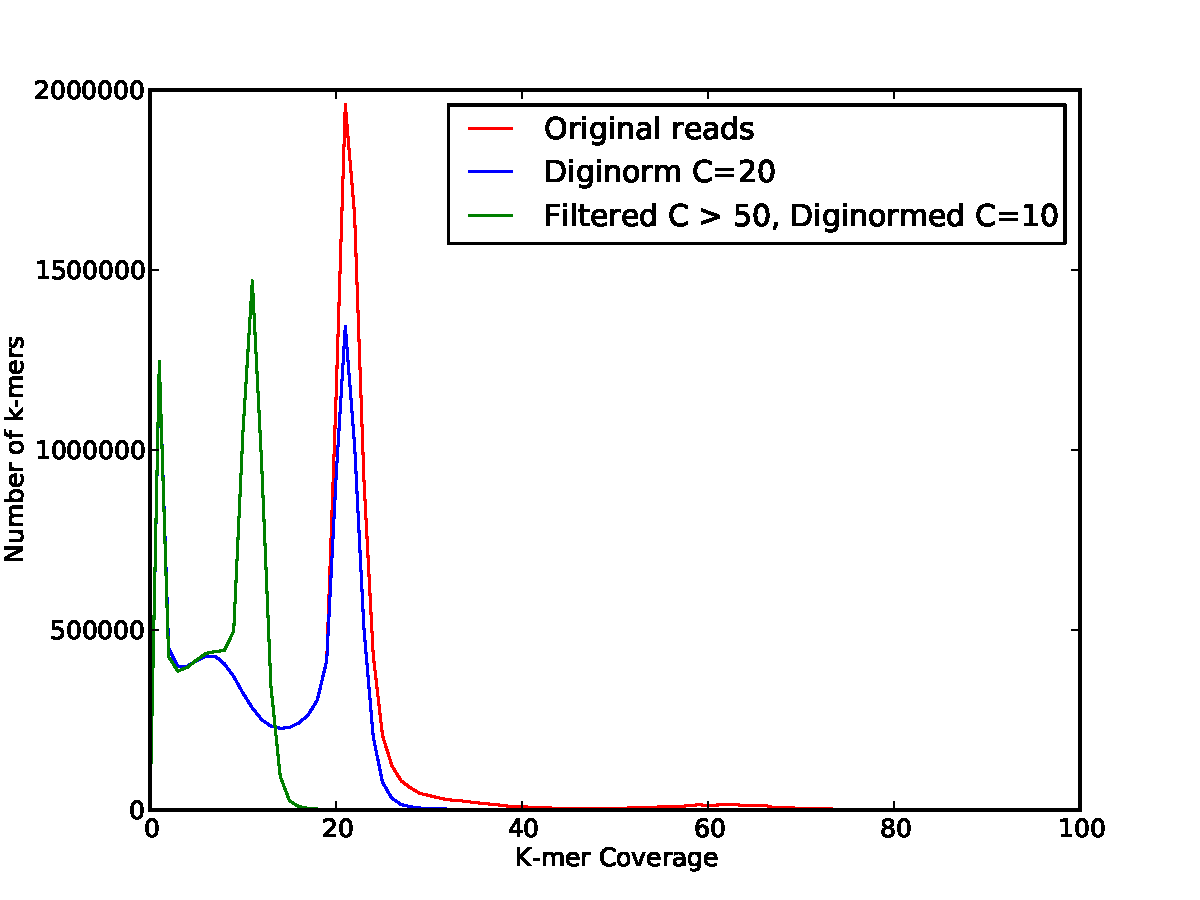
\includegraphics[width=\textwidth,height=\textheight,keepaspectratio]
{./figures/mockdiginormhist.pdf}}
\caption{ K-mer coverage of HMP mock community dataset before and
  after filtering approaches.}
\label{kmercoverage}
\end{figure}

\begin{figure}[ht]
\center{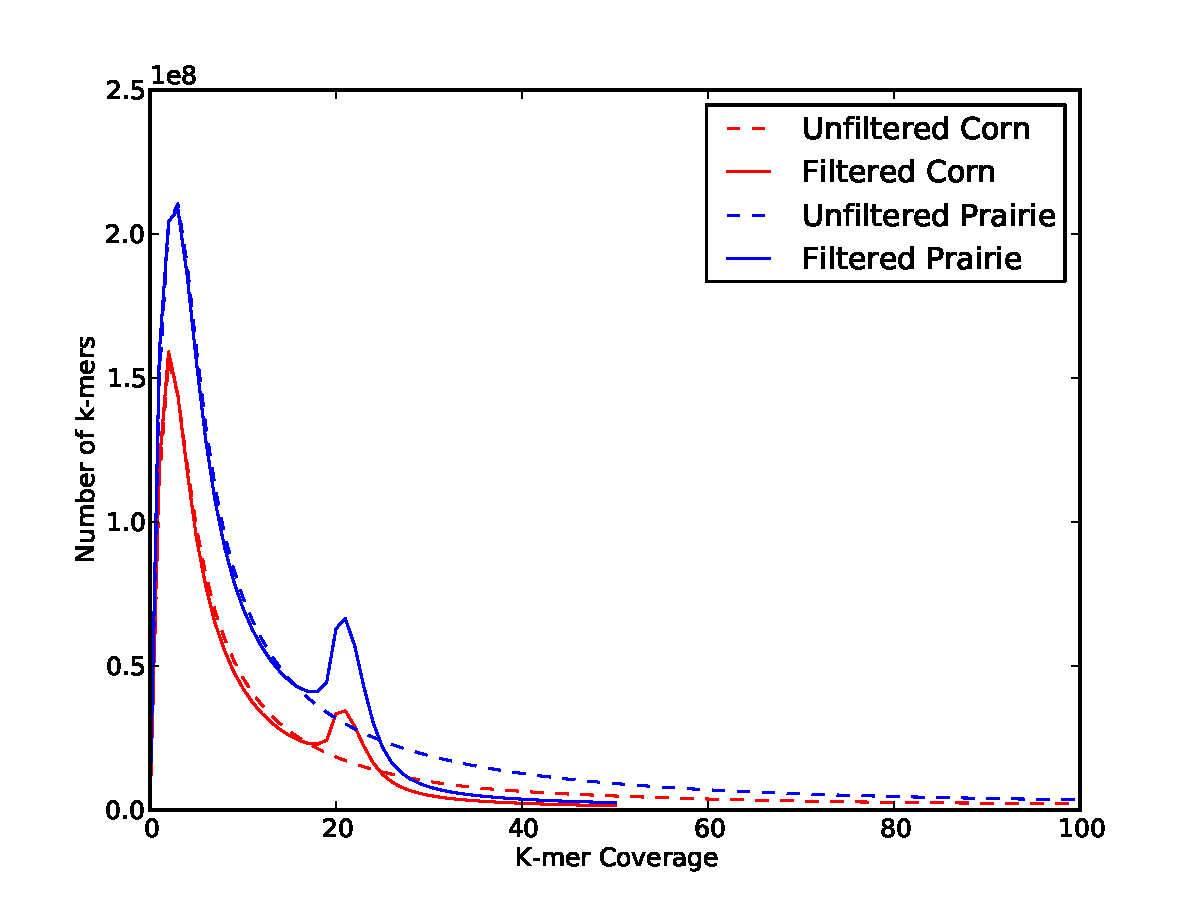
\includegraphics[width=\textwidth,height=\textheight,keepaspectratio]
{./figures/soildiginorm.pdf}}
\caption{K-mer coverage of Iowa corn and prairie metagenomes before
  and after filtering approaches.}
\label{diginormcoverage}
\end{figure}

\begin{figure}[ht]
\center{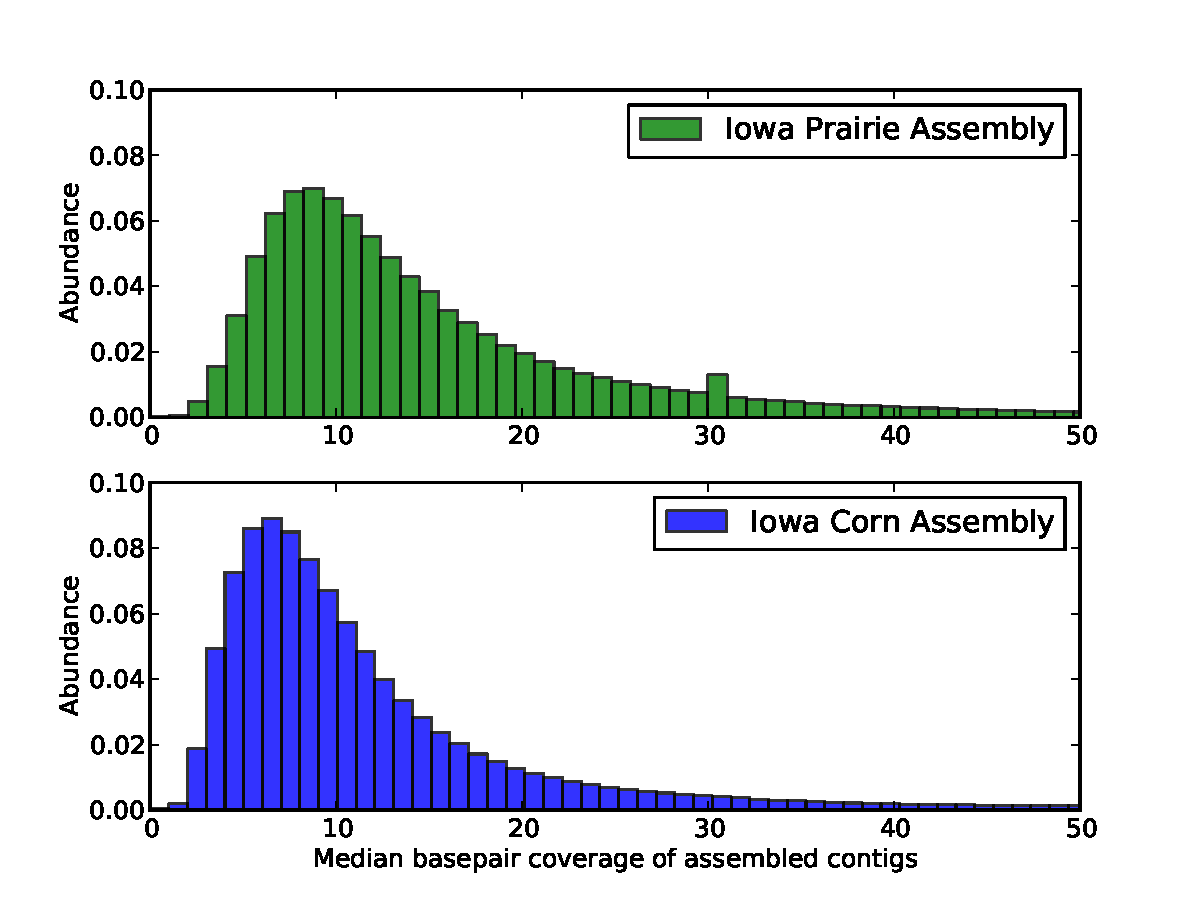
\includegraphics[width=\textwidth,height=\textheight,keepaspectratio]
  {./figures/assembly-coverage.pdf}}
\caption{Coverage (median basepair) distribution of assembled contigs
  from soil metagenomes.}
\label{soilassemblycoverage}
\end{figure}

\begin{figure}[ht]
\center{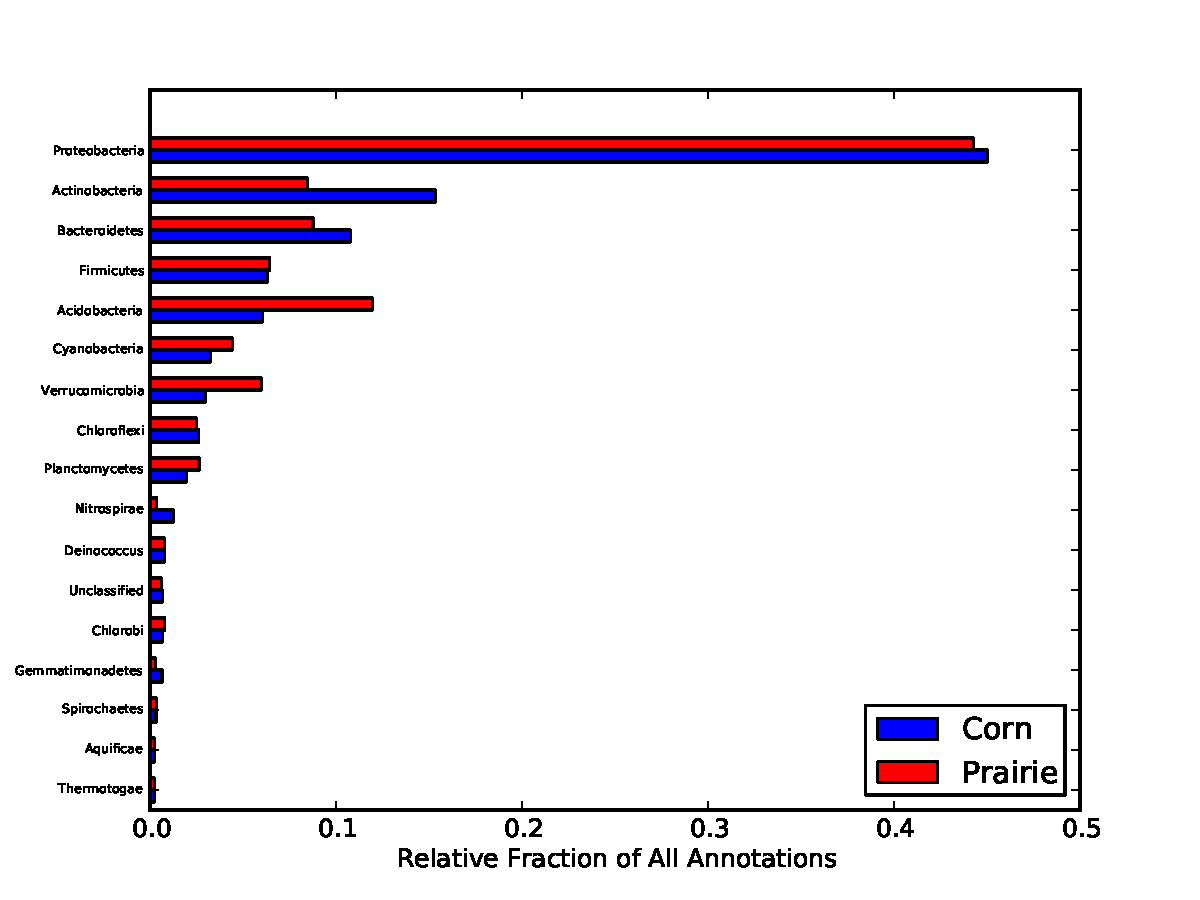
\includegraphics[width=\textwidth,height=\textheight,keepaspectratio]
  {./figures/phyla.pdf}}
\caption{Phylogenetic distribution from SEED subsystem annotations for
  Iowa corn and prairie metagenomes.}
\label{phyla}
\end{figure}

\begin{figure}[ht]
\center{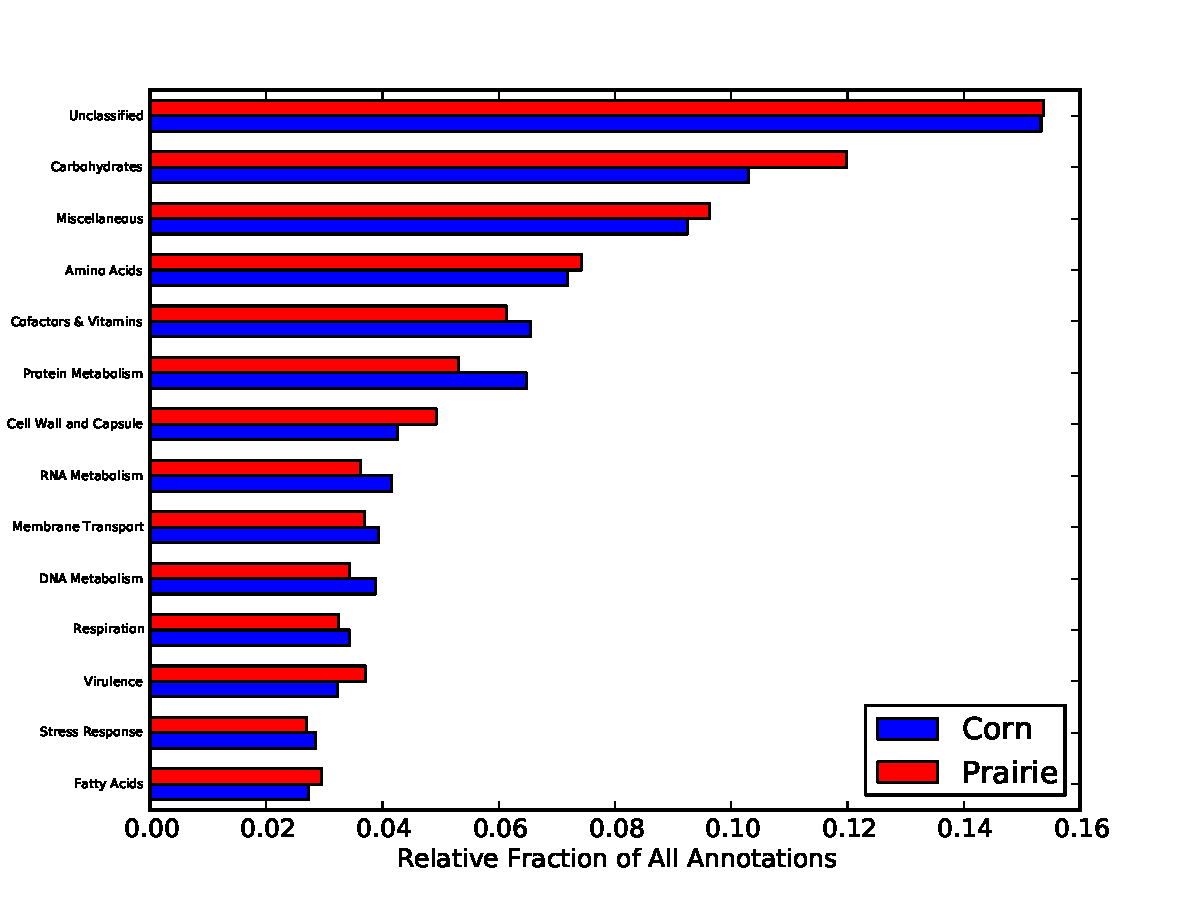
\includegraphics[width=\textwidth,height=\textheight,keepaspectratio]
  {./figures/subsystems.pdf}}
\caption{Functional distribution from SEED subsystem annotations for
  Iowa corn and prairie metagenomes.}
\label{subsystem}
\end{figure}

\end{document}
